\documentclass{standalone}

\usepackage{tikz}
\usepackage{circuitikz}

\tikzset{block/.style = {draw, fill=white, very thick, rectangle, minimum height=1cm, minimum width=2cm},
         lblock/.style={draw,fill=white,very thick, rectangle, minimum height=3cm, minimum width=1cm},
         sum/.style= {draw, fill=white, very thick, circle, node distance=0.5cm}}

         
\begin{document}
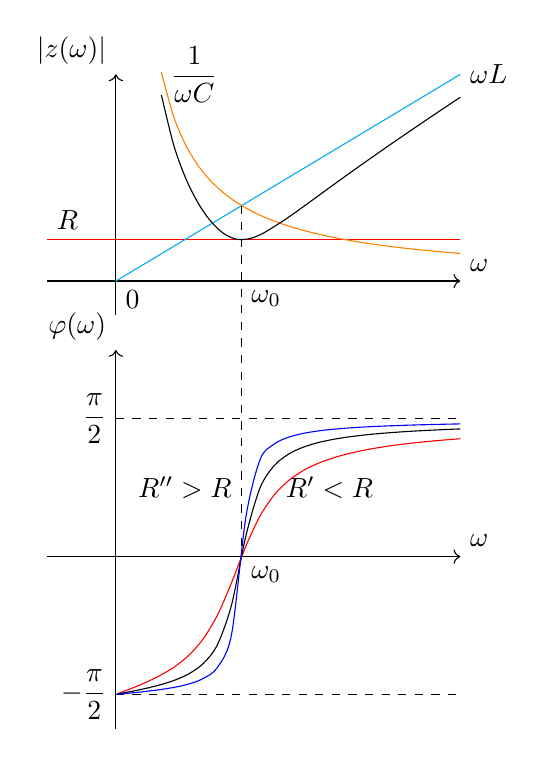
\begin{tikzpicture}[scale=1.75]
    \draw[->](-0.5,0)--(2.5,0)node[above right]{$\omega$};
    \draw[->](0,-0.25)--(0,1.5)node[above left]{$|z(\omega)|$};
    \draw[red](-0.5,0.3)node[above right, black]{$R$}--(2.5,0.3);
    \draw[cyan](0,0)node[below right, black]{$0$}--(2.5,1.5)node[right, black]{$\omega L$};
    \draw[orange]plot[smooth, domain=0.33:2.5](\x,{1/(2*\x)});
    \node[right]at(0.33,1.5){$\displaystyle\frac{1}{\omega C}$};
    \draw[black]plot[smooth, domain=0.33:2.5](\x,{(0.3^2+(3/5*\x-1/(2*\x))^2)^0.5});

    \draw[->](-0.5,-2)--(2.5,-2)node[above right]{$\omega$};
    \draw[->](0,-3.25)--(0,-0.5)node[above left]{$\varphi(\omega)$};
    \draw[dashed](0,-1)node[left]{$\displaystyle\frac{\pi}{2}$}--(2.5,-1);
    \draw[dashed](0,-3)node[left]{$-\displaystyle\frac{\pi}{2}$}--(2.5,-3);
    \draw[dashed](0.913,0.548)--(0.913,0)node[below right]{$\omega_0$}--(0.913,-2)node[below right]{$\omega_0$};
    \draw[red]plot[smooth,domain=0.01:2.5](\x,{2/pi*rad(atan((3/5*\x-1/(2*\x))/0.3))-2});
    \draw[black]plot[smooth,domain=0.01:2.5](\x,{2/pi*rad(atan(2*(3/5*\x-1/(2*\x))/0.3))-2});
    \draw[blue]plot[smooth,domain=0.01:2.5](\x,{2/pi*rad(atan(4*(3/5*\x-1/(2*\x))/0.3))-2});
    \node[]at(1.55,-1.5){$R'<R$};
    \node[]at(0.5,-1.5){$R''>R$};
\end{tikzpicture}
\end{document}